\section{\large Exercises}

\begin{exer}
    Solve the equation $e^{2x} - 6 e^x - 40 = 0$.
\end{exer}

\begin{exer}
    Find $\sin(A)$, $\cos(A)$, $\tan(A)$, $\sec(A)$, $\csc(A)$ and $\cot(A)$ in the below triangle.
    \begin{figure}[H]
        \center
        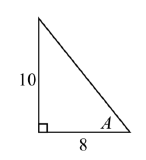
\includegraphics[width=3cm]{content/img.png}
    \end{figure}
\end{exer}

\begin{exer}
    In the following triangle, solve for the unknown sides and angle.
    \begin{figure}[H]
        \center
        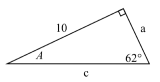
\includegraphics[width=5cm]{content/img_1.png}
    \end{figure}
\end{exer}

\begin{exer}
    An account grows exponentially from \$20,000 to \$30,000 in ten years.
    \begin{enumerate}
        \item Determine the average annual growth rate and use if to write an exponential function to model growth.
        \item Use the exponential model to find what the investment will be worth after 12 years and then when the investment will reach \$50,000.
    \end{enumerate}
\end{exer}